Z uporabo bitnih polj je mogoče predstaviti mnogo podatkovnih struktur. Primer uporabe bitnih polj je kompaktna predstavitev topologije dreves. Običajno je podatkovna struktura drevo sestavljeno iz vozlišč ter kazalcev (angl. \textit{pointers}). Vsako vozlišče shrani lastno vrednost ter kazalce na svoje otroke. Drevo z $n$-timi vozlišči potrebuje $O(n\log{n})$ bitov za shraniti topologijo drevesa. Kompaktna predstavitev topologije dreves zniža prostorsko zahtevnost na $2n+o(n)$ bitov. Za vsako vozlišče je potrebno predstaviti kazalec na vozlišče ter predstaviti, da je vozlišče bilo že obiskano, torej je potrebnih $2n$ bitov.

Pri tem obstajajo tri vrste kompaktne predstavitve dreves: Uravnoteženi oklepaji (angl. \textit{Balanced Parentheses} oziroma BP), Zaporedje eniških zapisov stopenj vozlišč po plasteh (angl. \textit{Level Order Unary Degree Sequence} oziroma LOUDS) in Zaporedje eniških zapisov stopenj vozlišč v globino (angl. \textit{Depth-First Unary Degree Sequence} oziroma DFUDS).
Naslednja definicija prikaže operacije, ki so potrebne za pravilno delovanje dreves.

\begin{defi}\label{def:drevo}
    Topologija podatkovne strukture drevo mora podpirati naslednje operacije:
    \begin{enumerate}
        \item $koren()$: vrne koren priponskega drevesa,
        \item $jeList(v)$: vrne »Da«, če je vozlišče list, sicer vrne »Ne«,
        \item $stOtrok(v)$: vrne število otrok vozlišča $v$,
        \item $otrok(v,i)$: vrne vozlišče $w$, ki je $i$-ti otrok vozlišča $v$,
        \item $prviOtrok(v)$: vrne vozlišče $w$, ki je prvi otrok vozlišča $v$,
        \item $nbrat(v)$: vrne vozlišče $w$, ki je naslednji brat od vozlišča $v$,
        \item $pbrat(v)$: vrne vozlišče $w$, ki je predhodni brat od vozlišča $v$,
        \item $star$\textit{š}$(v)$: vrne vozlišče $w$, ki je starš od vozlišča $v$,
        \item $globina(v)$ vrne število vozlišč na poti iz korena do vozlišča $v$,
        \item $lca(v,w)$: vrne najnižjega skupnega prednika od $v$ in $w$.
    \end{enumerate}
\end{defi}

S pomočjo teh operacij se je mogoče sprehoditi po drevesu in je možno implementirati ostale operacije dreves, na primer \texttt{vstavi}, \texttt{izbriši}, \texttt{najmanjši\_element} (v kopici) in ostale.

\subsection{Zaporedje eniških zapisov stopenj vozlišč po plasteh}\label{sec:LOUDS}

Prvi način zapisa topologije drevesa je zaporedje eniških zapisov stopenj vozlišč po plasteh (LOUDS). Drevo se predstavi kot bitno polje $B$ dolžine $2n+1$, pri čemer je $n$ število vozlišč v drevesu. Zapis drevesa se začne z nizom $10$, temu pa sledi zapis vsakega vozlišča. Vsako vozlišče $v$ je predstavljeno z nizom $1^o0$, pri je $o$ predstavlja število otrok posameznega vozlišča, torej se ena zapiše $o$-krat in nato eno ničlo, ki predstavlja konec vozlišča. Kot je razvidno iz imena predstavitve, so vozlišča obiskana po nivojih: vozlišča z isto globino so zaporedno predstavljana \cite{Navarro2016}.

Primer takega zapisa je predstavljen na Sliki \ref{fig:LOUDS}. Na sliki je koren drevesa predstavljen z $B[3,7]=11110$. Niz $B[3,7]$ vsebuje 4 bite z vrednostjo $1$, ker ima koren $4$ otroke.

\begin{figure}[htb]
    \begin{center}
        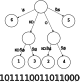
\includegraphics[width=.8\textwidth]{Slike/KokosSTLOUDR.png}
        \captionof{figure}[Primer predstavitve drevesa z metodo LOUDS za priponsko drevo besede »KOKOŠ$\$$«.]{Primer predstavitve drevesa z metodo LOUDS za priponsko drevo besede »KOKOŠ$\$$«.} 
        \label{fig:LOUDS}
    \end{center}
\end{figure}


Med izgradnjo kompaktne predstavitve se vsa vozlišča indeksira s številom $i$  med 1 in $n$. Število $i$ predstavlja zaporedno število obiskanega vozlišča, torej koren ima vrednost $1$, prvi otrok korena ima vrednost $2$ in tako dalje. Indeks se uporabi za shranjevanje vrednosti, ki so po navadi shranjene znotraj vozlišča. V Tabeli \ref{tab:LOUDSop} so predstavljene implementacije operacij s pomočjo predstavitve drevesa LOUDS. Vrednost $x$ predstavlja indeks vozlišča in se izračuna kot $x=izbira_0(B,v)+1$ \cite{Navarro2016}.

\begin{table}[htb]
    \centering
    \caption{Implementacija operacij drevesa v LOUDS.}
    \begin{tabular}{r|l}
\textbf{Operacija}& \textbf{Implementacija v LOUDS} \\\hline
         $koren()$& 3\\
         $jeList(v)$& $B[v]==0$\\
         $stOtrok(v)$& $naslednik_0(B,x)-x$\\
         $otrok(v,i)$& $izbira_0(B, rang_1(B, x - 1 + i))+1$\\
         $prviOtrok(v)$& $otrok(v,1)$\\
         $nbrat(v)$& $naslednik_0(B,v)+1$ \\
         $pbrat(v)$& $predhodnik_0(B,v-2)+1$ \\
         $star$\textit{š}$(v)$& $predhodnik_0(B,izbira_0(B,v-1))+1$ \\
         $globina(v)$& / \\
         $lca(v,w)$&  Algoritem \ref{alg:LOUDSlca}\\

    \end{tabular}
    \label{tab:LOUDSop}
\end{table}



 V Tabeli \ref{tab:LOUDSop} sta uporabljeni dve novi operaciji nad bitnimi polji: $naslednik_v(B,y)$ in $predhodnik_v(B,y)$, kjer je $v\in \{1,0\}$. Operacija predhodnik elementa $y$ najde element $x_i$ del zaporedja, za katerega velja $x_i \le y < x_{i+1}$ in $1\le i\le m$, kjer je $m$ število ponovitev $v$-ja v $B$. Operacija je implementirana kot
 $$predhodnik_v(B,y)=izbira_v(B,rang_v(B,y)),$$
 pri čemer je $v\in \{1,0\}$. Na podoben način je definirana tudi operacija naslednik. Operacija naslednik elementa $y$  najde položaj elementa $x_i$ v zaporedju $x_1\le x_2 \le \dots \le x_m$, pri čemer velja, da $x_{i-1}< y \le x_i$. Pri tem je implementirana kot
  $$naslednik_v(B,y)=izbira_v(B,rang_v(B,y-1)+1),$$
kjer je  $v\in \{1,0\}$. Zaporedje $x_1\le x_2 \le \dots \le x_n$ predstavlja vozlišča v zaporedju eniških zapisov stopenj vozlišč po plasteh. Torej operaciji predhodnik in naslednik vrneta začetni položaj predhodnega oziroma naslednjega vozlišča v bitnem polju $B$. Primer uporabe je operacija $stOtrok(v)$, ki izračuna število otrok, tako da odšteje položaj vozlišča $v$ v $B$ od položaja naslednjega bita z vrednostjo 0, ki predstavlja vozlišče $v$. Vse operacije razen operacije $globina$ in $lca$ so izvršene v konstantnem času, z uporabo dodatne podatkovne strukture za rang in izbiro. Pri tem je treba izgraditi podatkovno strukturo zgolj za $izbira_0$, saj operacija $izbira_1$ ni potrebna za pravilno delovanje operacij drevesa \cite{Navarro2016}.

 Operacija $globina$ ni podprta, saj LOUDS predstavitev ne omogoča učinkovitega iskanja. Pri tem pa velja, da $globina(u)\ge globina(v)$, če je $u>v$. S pomočjo tega dejstva se lahko implementira operacijo $lca$, kot je prikazano v Algoritmu \ref{alg:LOUDSlca} \cite{Navarro2016}.
 
 \begin{algorithm}[hbt]

\Vhod{Bitno polje $B$, vozlišča $v$ in $w$}
\Izhod{Vozlišče $u$}
\caption{Operacija $lca(v,w)$ (LOUDS)}\label{alg:LOUDSlca}
{
    \While{$v\ne w$}{
        \Ce{$v>w$}
            {$v$<-$star$\textit{š}$(B,v)$}
            \Sicer{$w$<-$star$\textit{š}$(B,w)$}
    }
    \Vrni{$v$}    
    
}
\end{algorithm}


\subsection{Uravnoteženi oklepaji}\label{sec:oklepaji}

Naslednji način zapisa topologije drevesa je zapis z zaporedjem uravnoteženih oklepajev (BP). Drevo se predstavi, kot bitno polje $B$ dolžine $2n$, pri čemer je $n$ število vozlišč v drevesu. Zaporedje se zgradi s pomočjo pregleda v globino. Ko je vozlišče prvič obiskano se, na konec do sedaj zapisane sekvence, zapiše '('. Uklepaj je v bitnem polju predstavljen s številom $0$. Ko se zapiše celotno poddrevo vozlišča, pa se na konec sekvence zapiše ')'. Zaklepaj pa je v bitnem polju zapiše s številom $1$. Primer priponskega drevesa predstavljenega z uporabo zaporedja uravnoteženih oklepajev je prikazan na Sliki \ref{fig:BP} \cite{Navarro2016}.

\begin{figure}[htb]
    \begin{center}
        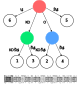
\includegraphics[width=0.8\textwidth]{Slike/KokosSTBP.png}
        \captionof{figure}[Primer predstavitve drevesa z metodo BP za priponsko drevo besede »KOKOŠ$\$$«.]{Primer predstavitve drevesa z metodo BP za priponsko drevo besede »KOKOŠ$\$$«.} 
        \label{fig:BP}
    \end{center}
\end{figure}

Torej je vsako vozlišče je predstavljeno kot par '(' in ')'. Tako je mogoče definirati sledeče operacije nad oklepaji: $odpri$, $zapri$, $vi$\textit{š}$ek$ ter $oklepa$. Operacija $vi$\textit{š}$ek(B,i)$ vrne število '(', ki niso bili še zaprti in je
$$
    vi\textit{š}ek(B,i)=rang_0(B,i)-rang_1(B,i)=2rang_0(B,i)-i.
$$
Operacija $odpri(B,i)$ vrne položaj '(', ki odpre ')' na $i$-tem mestu v $B$. Operacijo $odpri(B,i)$ se lahko definira tudi, tako da vrne prvi $j>i$, pri čemer $vi$\textit{š}$ek(B,j)=vi$\textit{š}$ek(B,i)-1$. Podobno operacija $zapri(B,i)$  vrne položaj ')', ki zapre '(' na $i$-tem mestu v $B$. Z uporabo operacije $vi$\textit{š}$ek$ je operacija $zapri$ definirana, tako da vrne največji $j<i$, pri čemer je $vi$\textit{š}$ek(B,j)=vi$\textit{š}$ek(B,i)+1$. Operacija $oklepa(B,i)$ vrne položaj $j$ od '(' v bitem polju $B$, pri čemer velja, da $j<i<zapri(B,j)$. Z uporabo operacije $vi$\textit{š}$ek$ operacija $oklepa(B,i)$ vrne položaj največjega $j<i$, pri čemer je $vi$\textit{š}$ek(B,j-1)=vi$\textit{š}$ek(B,i)-2$
 \cite{Navarro2016}.

Pravilno delovanje drevesa, ki je predstavljen z uporabo BP, zahteva še operacije o višku nad odseki bitnega polja $B$. Te operacije so sledeče: $rmq$, $rMq$, $minizbira$ in $min$\textit{š}$tetje$. Operacija $rmq(B,i,j)$ (angl. \textit{range minimum query}) vrne položaj $k$, kjer je $i\le k\le j$, $vi$\textit{š}$ek(B,k)$ je najnižji višek v območju med $i$ in $j$ ter $k$ je prvi pojav najnižjega viška na tem območju. Podobno je definirana tudi operacija $rMq(B,i,j)$ (angl. \textit{range maximum query}), ki pa vrne položaj $k$, pri čemer je $i\le k\le j$ in $vi$\textit{š}$ek(B,k)$ je najvišji višek v območju med $i$ in $j$ ter $k$ je prvi pojav najvišjega viška na območju. Operacija $minizbira(B,i,j,t)$ vrne položaj $t$-tega pojava najmanjšega viška na območju med $i$ in $j$. Operacija $min$\textit{š}$tetje(B,i,j)$ pa vrne število pojav najnižjega viška na območju med $i$ in $j$ \cite{Navarro2016}.

Vse predstavljene operacije (razen operacije $vi$\textit{š}$ek$, ki potrebuje $O(1)$ časa za izvajanje) se lahko implementira s časovno zahtevnostjo $O(\log{n})$. Pri tem pa je potrebno zgraditi dodatno podatkovno strukturo rmM-drevo (angl. \textit{range minumum maximum tree}), ki je lahko shranjeno z $O(n/\log{n})=o(n)$ dodatnimi biti. Podatkovna struktura razdeli bitno polje $B$ na $\frac{n}{b}$ veder velikosti $b$ ter za vsako vedro se ustvari list rmM-drevesa. Drevo je levo poravnano in se lahko zapiše kot polje vozlišč (podobno kot podatkovna struktura kopica). Torej so otroci $i$-tega vozlišča na $2i$-tem in $2i+1$-vem mestu v polju ter starš $i$-tega vozlišča se nahaja na $\left\lfloor\frac{i}{2}\right\rfloor$-mestu. Vsako vozlišče v drevesu hrani štiri podatke: $e$ razlika viška med začetkom in koncem pokritega območja, $m$ najmanjši relativni višek v območju, $M$ največji relativni višek na območju in $n$ število najmanjših viškov na območju, ki ga pokriva vozlišče. Pri tem vozlišče pokriva celotno območje, ki ga pokrivata oba otroka, in listi pokrivajo zgolj eno vedro dolžine $b$. Torej koren drevesa pokriva celotno bitno polje $B$. Vse predstavljene operacije so implementirane s pomočjo sprehoda po rmM-drevesu 
\cite{Navarro2016}.

Podobno kot pri predstavitvi drevesa LOUDS, tudi predstavitev BP potrebuje dodatno podatkovno strukturo za operaciji $izbira$ in $rang$. Pri tem sta potrebni zgolj podatkovni strukturi za $0$, saj  operaciji $rang_1$ in $izbira_1$ nista potrebni za pravilno delovanje drevesa v tej predstavitvi. Podatkovni strukturi potrebujeta vsaka $o(n)$ dodatnih bitov in operaciji se izvršita v konstantnem času.

\begin{table}[htb]
    \centering
      \caption{Implementacija operacij drevesa z BP}
    \begin{tabular}{r|l}
\textbf{Operacija}& \textbf{Implementacija v BP} \\\hline
         $koren()$& 1\\
         $jeList(v)$& $B[v]==0 \wedge B[v+1]==1$\\
         $stOtrok(v)$& $min$\textit{š}$tetje(B,v,zapri(B,v)-2)$\\
         $otrok(v,i)$&  $minizbira(B,v,zapri(B,v)-2,i)+1$\\
         $prviOtrok(v)$& $v+1$\\
         $nbrat(v)$& $zapri(B,v)+1$ \\
         $pbrat(v)$& $odpri(B,v-1)$ \\
         $star$\textit{š}$(v)$& $oklepa(B,x)$ \\
         $globina(v)$& $2\cdot rang_0(B,v)-v$ \\
         $lca(v,w)$&  $okelpa(B,rmq(B,v,w)+1);v<w$\\
    \end{tabular}  
    \label{tab:BPop}
\end{table}

V Tabeli \ref{tab:BPop} so prikazane implementacije operacij, ki so potrebne za pravilno delovanje drevesa. Indeks $x=izbira_0(B,v)$ je uporabljen za pridobiti dodatne informacije o vozlišču, saj vrednost $v$ predstavljata položaja '(' v zaporedju $B$, ne pa indeksa v tabeli z dodatnimi informacijami o vozlišču.

Zapis topologije drevesa s BP omogoča dodatne operacije. Primer operacije je oštevilčenje in iskanja listov drevesa, kar je storjeno s pomočjo posplošitve operacije rang in izbiro na poljubno dolge nize. Ker imajo listi imajo obliko »()« (oziroma $01$, ko so zapisani v bitnem polju $B$), se lahko implementirata operaciji $rang_{01}(B,i)$ in $izbira_{01}(B,i)$. Operaciji potrebujeta konstanten čas, da se izvedeta, saj se lahko izgradi podobno dodatno strukturo, kot za osnovno verzijo ranga in izbire.


\subsection{Zaporedje eniških zapisov stopenj vozlišč v globino}\label{sec:DFUDS}

Zadnja predstavitev topologije drevesa je zaporedje eniških zapisov stopenj vozlišč v globino (DFUDS). Predstavitev omogoča preprostejše implementacije operacij ter posledično manjše dodatne podatkovne strukture, za razliko od zapisa z zaporedjem uravnoteženih oklepajev. Pri tem pa omogoča hitrejše implementacije nekaterih operacij v primerjavi, z uporabo zaporedja eniških zapisov stopenj vozlišč po plasteh. Primer zapisa topologije drevesa z DFUDS je prikazan na Sliki \ref{fig:DFUDS}.

\begin{figure}[htb]
    \begin{center}
        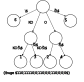
\includegraphics[width=.8\textwidth]{Slike/KokosSTDFUDS.png}
        \captionof{figure}[Primer predstavitve drevesa z metodo DFUDS za priponsko drevo besede »KOKOŠ$\$$«.]{Primer predstavitve drevesa z metodo DFUDS za priponsko drevo besede »KOKOŠ$\$$«.} 
        \label{fig:DFUDS}
    \end{center}
\end{figure}

Drevo je predstavljeno z bitnim poljem $B[1,2n+2]$. Zapis temelji na uporabi zaporedja uravnoteženih oklepajev in zapisu stopenj vozlišč, zato je potrebno dodati na začetek bitnega polja $B[1,3]=110$. Zatem pa so zapisane stopnje vozlišč, kot zaporedje $1^o0$ pri čemer $o$ je število otrok vozlišča. Zapis je zgrajen z uporab pregleda v globino. Vsa vozlišča imajo indeks, ki je zaporedno število obiskanega vozlišča.

\begin{table}[htb]
    \centering
    \caption{Implementacija operacij drevesa z DFUDS}
    \begin{tabular}{r|l}
\textbf{Operacija}& \textbf{Implementacija v DFUD}S \\\hline
         $koren()$& 4\\
         $jeList(v)$& $B[v]==0$\\
         $stOtrok(v)$& $naslednik_0(B,v)-v$\\
         $otrok(v,i)$& $zapri(B, naslednik_0(B, v) - i)+1$\\
         $prviOtrok(v)$& $naslednik_0(B,v)+1$\\
         $nbrat(v)$& $iskanjeNaprej(B,v-1,-1)+1$ \\
         $pbrat(v)$& $zapri(B,odpri(B,v-1)+1)+1$ \\
         $star$\textit{š}$(v)$& $predhodnik_0(B,izbira_1(B,v-1))+1$ \\
         $globina(v)$& / \\
         $lca(v,w)$&  $star$\textit{š}$(B,rmq(naslednik_0(B,w),v+1)+1);v<w$\\

    \end{tabular}
    \label{tab:DFUDSop}
\end{table}


V Tabeli \ref{tab:DFUDSop} so predstavljene implementacije operaciji nad drevesom implementirane z DFUDS. Indeks  $x=izbira_0(B,v)+1$ je uporabljen za shranjevanje dodatnih informacij o vozlišču, saj je vozlišče $v$ predstavljeno s položajem vozlišča v bitnem polju $B$. V tabeli je vidno, da operacija $globina(v)$ ni podprta, saj ni mogoče implementirati te operacije brez sprehoda od vozlišča $v$ do korena ter pri tem šteti potrebne korake. Operacija $lca(v,u)$ je lahko implementirana brez sprehoda po drevesu za razliko od implementacije z LOUDS.

Pri implementaciji operacije $nbrat(v)$ pa je prisotna operacija $iskanjeNaprej(B,i,d)$. Operacija omogoča iskanje prvega pojava viška, ki je za $d$ večji od viška na $i$-tem mestu v bitnem polju $B$. Operacija je definirana kot
$$
    iskanjeNaprej(B,i,d)=\min\{j>i; vi\textit{š}ek(B,j)=vi\textit{š}ek(B,i)+d\}\cup\{n+1\}.
$$
Operacija $iskanjeNaprej$ je lahko implementirana s pomočjo uporabe $rmM$-drevesa in potrebuje $O(\log{n})$ časa, da se izvrši. Implementirana je s pomočjo sprehoda po $rmM$-drevesu in uporabo viška na intervalu pokritega z vozliščem $v$ ($rmM[v].e$, pri čemer je polje $rmM$ predstavitev $rmM$-drevesa) in najmanjšega relativnega viška na intervalu pokritim z vozliščem $v$ ($rmM[v].m$, pri čemer polje $rmM$ je predstavitev $rmM$-drevesa).

Vse operacije, ki temeljijo na operaciji $rang$ in $izbira$, se izvršijo v $O(1)$ času. Operacije, ki pa temeljijo na $rmM$-drevesu, pa potrebujejo $O(\log{n})$ časa. Pri tem so potrebne dodatne podatkovne strukture za $izbira_1$, $izbira_0$, $rang$ ter $rmM$-drevo, pri čemer vsaka potrebuje $o(n)$ dodatnih bitov. Pri tem je mogoče zmanjšati prostorsko zahtevnost $rmM$-drevesa, tako da se shranita zgolj polji $e$ in $m$. Tako se razpolovi prostorsko zahtevnost drevesa, ki pa še vedno zahteva $o(n)$ dodatnih bitov, brez škode za implementacijo operacij drevesa. Tega ni mogoče storiti v BP, saj $rMq(B,i,j)$ se uporablja pri implementaciji dodatnih operaciji, primer take operacije je $najglobljeVozli$\textit{šč}$e(v)$, ki vrne najgloblje vozlišče v poddrevesu s korenom $v$.

Podobno kot pri predstavitvi drevesa z uporabo zaporedja uravnoteženih oklepajev je mogoče implementirati dodatne operacije nad listi. Za razliko od uravnoteženih oklepajev, kjer ima list obliko $10$, ima list obliko $00$ v zaporedju eniških stopenj v globino. Prva $0$ predstavlja konec predhodnega vozlišča. Tako je možno implementirati $rang_{00}$ in $izbira_{00}$, ki omogočata iskanje listov v drevesu. Pri tem sta potrebi popravljeni podatkovni strukturi za $rang$ in $izbiro$, ki pa potrebujeta vsaka $o(n)$ dodatnih bitov ter  še vedno omogočata konstanten čas izvajanja posplošenih operacij $rang_{00}$ in $izbira_{00}$.  